\documentclass{article}
\usepackage[utf8]{inputenc}
\usepackage{geometry}
\usepackage{tikz}
\usetikzlibrary{shapes,arrows,positioning,fit,backgrounds}
\geometry{a4paper, margin=1in}

\begin{document}

\section*{10. AI-driven Crop Yield Prediction}

\noindent \textbf{Description:} Develop an application that utilizes machine learning algorithms to predict crop yields based on historical and real-time data.

\vspace{1em}

\noindent \textbf{Objective:} Provide accurate predictions for better planning.

\vspace{1em}

\noindent \textbf{Recommended UML Diagrams:} Component Diagram, Activity Diagram.

\section*{Component Diagram}

\begin{center}
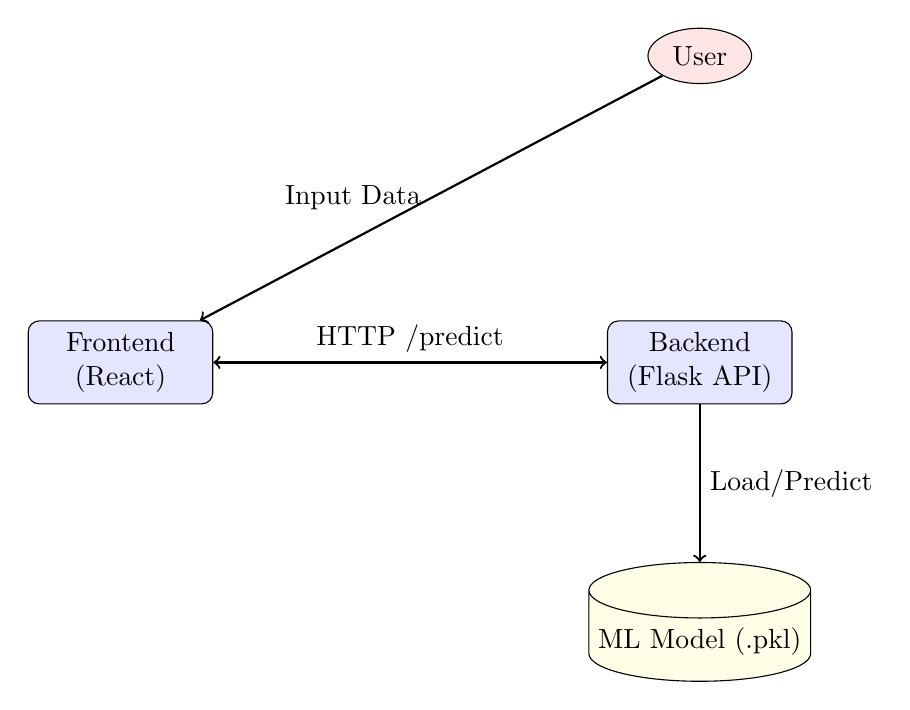
\begin{tikzpicture}[
    node distance=2cm,
    block/.style={rectangle, draw, fill=blue!10, text width=6em, text centered, rounded corners, minimum height=3em},
    cloud/.style={draw, ellipse, fill=red!10, node distance=3cm, minimum height=2em},
    database/.style={cylinder, draw, shape border rotate=90, aspect=0.25, fill=yellow!10}
]

% Nodes
\node [block] (frontend) {Frontend (React)};
\node [block, right=of frontend, xshift=3cm] (backend) {Backend (Flask API)};
\node [database, below=of backend] (model) {ML Model (.pkl)};
\node [cloud, above=of backend] (user) {User};

% Edges
\path [draw, ->, thick] (user) -- node [left] {Input Data} (frontend);
\path [draw, <->, thick] (frontend) -- node [above] {HTTP /predict} (backend);
\path [draw, ->, thick] (backend) -- node [right] {Load/Predict} (model);

\end{tikzpicture}
\end{center}

\section*{Activity Diagram}

\begin{center}
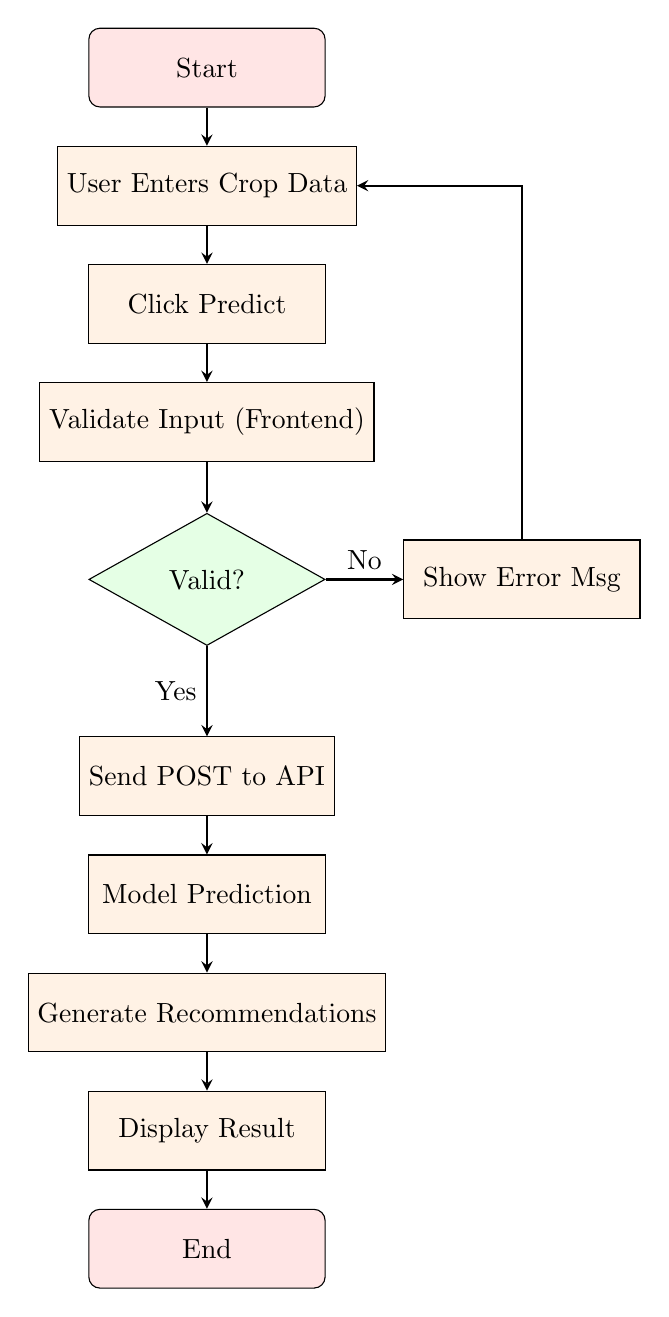
\begin{tikzpicture}[auto, node distance=1.5cm,
    startstop/.style = {rectangle, rounded corners, minimum width=3cm, minimum height=1cm,text centered, draw=black, fill=red!10},
    process/.style = {rectangle, minimum width=3cm, minimum height=1cm, text centered, draw=black, fill=orange!10},
    decision/.style = {diamond, minimum width=3cm, minimum height=1cm, text centered, draw=black, fill=green!10},
    arrow/.style = {thick,->,>=stealth}
]

% Nodes
\node (start) [startstop] {Start};
\node (input) [process, below of=start] {User Enters Crop Data};
\node (submit) [process, below of=input] {Click Predict};
\node (validate) [process, below of=submit] {Validate Input (Frontend)};
\node (decide1) [decision, below of=validate, yshift=-0.5cm] {Valid?};
\node (request) [process, below of=decide1, yshift=-1cm] {Send POST to API};
\node (predict) [process, below of=request] {Model Prediction};
\node (rules) [process, below of=predict] {Generate Recommendations};
\node (display) [process, below of=rules] {Display Result};
\node (end) [startstop, below of=display] {End};

\node (error) [process, right of=decide1, xshift=2.5cm] {Show Error Msg};

% Edges
\draw [arrow] (start) -- (input);
\draw [arrow] (input) -- (submit);
\draw [arrow] (submit) -- (validate);
\draw [arrow] (validate) -- (decide1);
\draw [arrow] (decide1) -- node[anchor=east] {Yes} (request);
\draw [arrow] (decide1) -- node[anchor=south] {No} (error);
\draw [arrow] (error) |- (input);
\draw [arrow] (request) -- (predict);
\draw [arrow] (predict) -- (rules);
\draw [arrow] (rules) -- (display);
\draw [arrow] (display) -- (end);

\end{tikzpicture}
\end{center}

\end{document}
